The proposed implementation of the ECDAR code generator is split up
in two parts. The first part is a framework of abstract classes, implementing
in as much detail as possible the single parts of ECDAR specifications
(i.e. edges, locations, TIOA). The second is the actual code generation.
Our code generator generates sources which inherit from the abstract
framework to minimize the amount of code that needs actually to be
generated. This means that nearly all design decisions have been made
prior to generating code, reducing space for possible errors. This
section describes our implemented subset of ECDAR and the code generator
in detail. 


\subsection{Presumptions and Resulting Motivations\label{implementation-presumptions}}

Our implementation represents only a subset of actual ECDAR. Currently,
the implementation assumes only one clock per automaton. Also, we
assume the specification to be valid, since there are other tools
that verify correctness%
\footnote{\href{}{http://people.cs.aau.dk/adavid/ecdar/}%
}.

Additionally, the only operator we implement is the parallel composition
operator. Let $M$ be the type ECDAR specification. Then all operators
in ECDAR are of type $M\rightarrow M\rightarrow M$. Other than for
the majority of operators, which refine the specification, it is impractical
to implement parallel composition as a model-to-model transformation,
since it produces the cross-product of two models. \cite{david_compositional_2012}
These models are size $|M|^{2}$ and generating code for them would
consume a large amount of memory and complexity. This would be inappropriate
for an embedded system. We elaborate on this further in Sec. \ref{implementation-framework}.

ECDAR specifications are written on the assumption of the synchrony
hypothesis (see Sec. \ref{background-ecdar}). \cite{david_compositional_2012}
This is an important property for code generation, as reasoning about
time differences in execution becomes unnecessary for the developer.
However, we still kept overhead low to achieve reasonable fast performance.

To produce feasible code that would be able to run on embedded systems,
we targeted Real-Time Java (Java RTS)%
\footnote{\href{}{http://www.oracle.com/technetwork/java/javase/tech/index-jsp-139921.html}%
}. Java RTS was designed to improve upon standard Java in terms of
timing accuracy an real-time embedded systems.


\subsection{The ECDAR Framework \label{implementation-framework}}

\begin{figure}
\begin{centering}
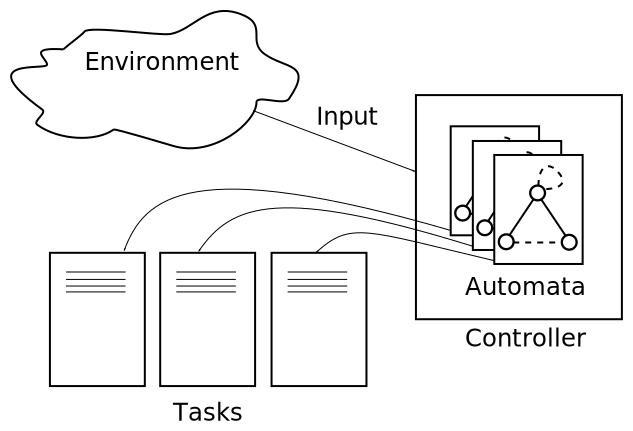
\includegraphics[scale=0.5]{images/ecdar_architecture}
\par\end{centering}

\caption{Schematic of the architecture of our ECDAR implementation.}
\end{figure}


The architecture we chose is based upon Amnell et al.\cite{amnell_code_2002}
with some modifications. Communication between automata happens through
input generated by uncontrollable edges -- there are no shared variables
(see Sec. \ref{background-tioa}). Input is processed by a controller
object, which initializes automata and notifies automata about input.

We require multiple automata to execute in quasi-parallel. Therefore,
we do not queue tasks. Since the automata are moved to classical threading
architecture, we do not require multiple processor units. Instead,
the controller and each automaton run in separate threads. Since there
is no communication between automata directly, we can minimize synchronizing
so that nearly no waiting is required.

The following overview will give further implementation details on
each component of ECDAR as we implemented it:


\subsubsection{Locations}

Each location is a associated with a task. Task execution is moved
to a separate thread. Location is implemented as a class holding an
array of controllable and uncontrollable edges that point away from
it.


\subsubsection{Edges}

An edge holds a reference to the location which the parent automaton
will be at after traversing this very edge. Edges can be asked if
they will be available at a given time. This is implemented to enable
lazy waiting in the automaton's traversal checker. Each edge is associated
with some input. If an edge is controllable, it will be triggered
if the automaton is notified at this input. If it is uncontrollable,
it will send its input to the controller. Furthermore, edges have
access to the clock of the parent automaton to reset it appropriately.

The implementation makes a class-wise distinction between controllable
and uncontrollable edges and hard-codes the behavior for given input.
Such hard-coded features are e.g. notifying the controller on traversing
an uncontrollable edge.


\subsubsection{TIOA}

The implementation of timed I/O automata holds a set of locations
and a reference to the location it is currently at. The TIOA is executed
by a thread that keeps checking for available edges and traverses
along these, as soon as they become enabled. To check if an edge is
available, let $E_{s\rightarrow t}$ be an edge where $s,\, t$ are
start and target locations respectively. Furthermore, let $g(E)$
be a function evaluating the guard of an edge $E$ and $I(l)$ a function
evaluating the invariant of a location $l$. Our implementation uses
$g'(E_{s\rightarrow t})=g(E_{s\rightarrow t})\wedge I(t)$ to check
if $E_{s\rightarrow t}$ is available.

Additionally, the automaton has the ability to return the current
local clock state (see \ref{implementation-presumptions}) and to
reset the clock. We use the same notion of clocks as \cite{amnell_code_2002},
where time on the local clock is the difference between the current
time on the system clock and the time the local clock was started.
Resetting the local clock means to use the current system clock time
as the new start time.


\subsubsection{Controller}

The controller holds all automata given in the specification, executes
them initially in quasi-parallel and notifies automata about input
from the environment. It is a singleton, accessible in a static fashion.
This property is useful for uncontrollable edges that need to notify
the controller about input.


\subsection{Walk-through Example}

% We may need an example specification here, some two-locations-two-edges thingy.


\subsection{Code Generation \label{implementation-code-generation}}

*Draft* 

In our implementation we generate executable Java code based on ECDAR models. The method we chose to use is the model-to-text transformation method.


We chose to use model-to-text instead of model-to-model transformations
because of the complexity (a lot of meta classes) and also because
of the limited scope of the project. % Rewrite this!
